\documentclass{beamer}
%%%%%%%%%%%%%%%%%%%%%%%%%%%%%%%%%%%%%%%%%%%%%%%%%%%%%%%%%%%%%%%%%%%%%%%%%%%%%%%%%%%%%%%%%%%%%%%%%%
\setbeamertemplate{navigation symbols}{}
\usepackage{beamerthemeshadow}
\usefonttheme{serif}
%%%%%%%%%%%%%%%%%%%%%%%%%%%%%%%%%%%%%%%%%%%%%%%%%%%%%%%%%%%%%%%%%%%%%%%%%%%%%%%%%%%%%%%%%%%%%%%%%%
\usepackage{graphicx}
\graphicspath{ {res/} }
%%%%%%%%%%%%%%%%%%%%%%%%%%%%%%%%%%%%%%%%%%%%%%%%%%%%%%%%%%%%%%%%%%%%%%%%%%%%%%%%%%%%%%%%%%%%%%%%%%
\usepackage{polyglossia}
\setdefaultlanguage{armenian}
\setotherlanguages{english}
\usepackage{fontspec}
\newfontfamily\armenianfont{DejaVu Sans}
%%%%%%%%%%%%%%%%%%%%%%%%%%%%%%%%%%%%%%%%%%%%%%%%%%%%%%%%%%%%%%%%%%%%%%%%%%%%%%%%%%%%%%%%%%%%%%%%%%
\usepackage{minted}
\setmonofont{Consolas}
%%%%%%%%%%%%%%%%%%%%%%%%%%%%%%%%%%%%%%%%%%%%%%%%%%%%%%%%%%%%%%%%%%%%%%%%%%%%%%%%%%%%%%%%%%%%%%%%%%
\usepackage{xltxtra}
\usepackage{hyperref}
%%%%%%%%%%%%%%%%%%%%%%%%%%%%%%%%%%%%%%%%%%%%%%%%%%%%%%%%%%%%%%%%%%%%%%%%%%%%%%%%%%%%%%%%%%%%%%%%%%
\usetheme{Luebeck}
\usecolortheme{crane}
%%%%%%%%%%%%%%%%%%%%%%%%%%%%%%%%%%%%%%%%%%%%%%%%%%%%%%%%%%%%%%%%%%%%%%%%%%%%%%%%%%%%%%%%%%%%%%%%%%

\begin{document}

\title[Visitor]{Նախագծման Ձևանմուշներ։ Visitor}
\author[Հրաչյա Թանդիլյան\copyright]{Հրաչյա Թանդիլյան}
\date{2020}

%-------------------------------------------------------------------------------------------------
\begin{frame}
\titlepage
\end{frame}
%-------------------------------------------------------------------------------------------------

\section{Նպատակը}
%-------------------------------------------------------------------------------------------------
\begin{frame}\frametitle{Visitor}
\begin{block}{Նպատակը}
    Տվյալ օբյեկտի համար տրամադրել այնպիսի փոխարինող, որը կվերահսկի նրան դիմումը:
\end{block}
\vfill
Նաև հայտնի է որպես
\begin{itemize}
    \item Surrogate
\end{itemize}
\end{frame}
%-------------------------------------------------------------------------------------------------

\subsection{Մոտիվացիան}
%-------------------------------------------------------------------------------------------------
\begin{frame}\frametitle{Մոտիվացիան}
\begin{center}
    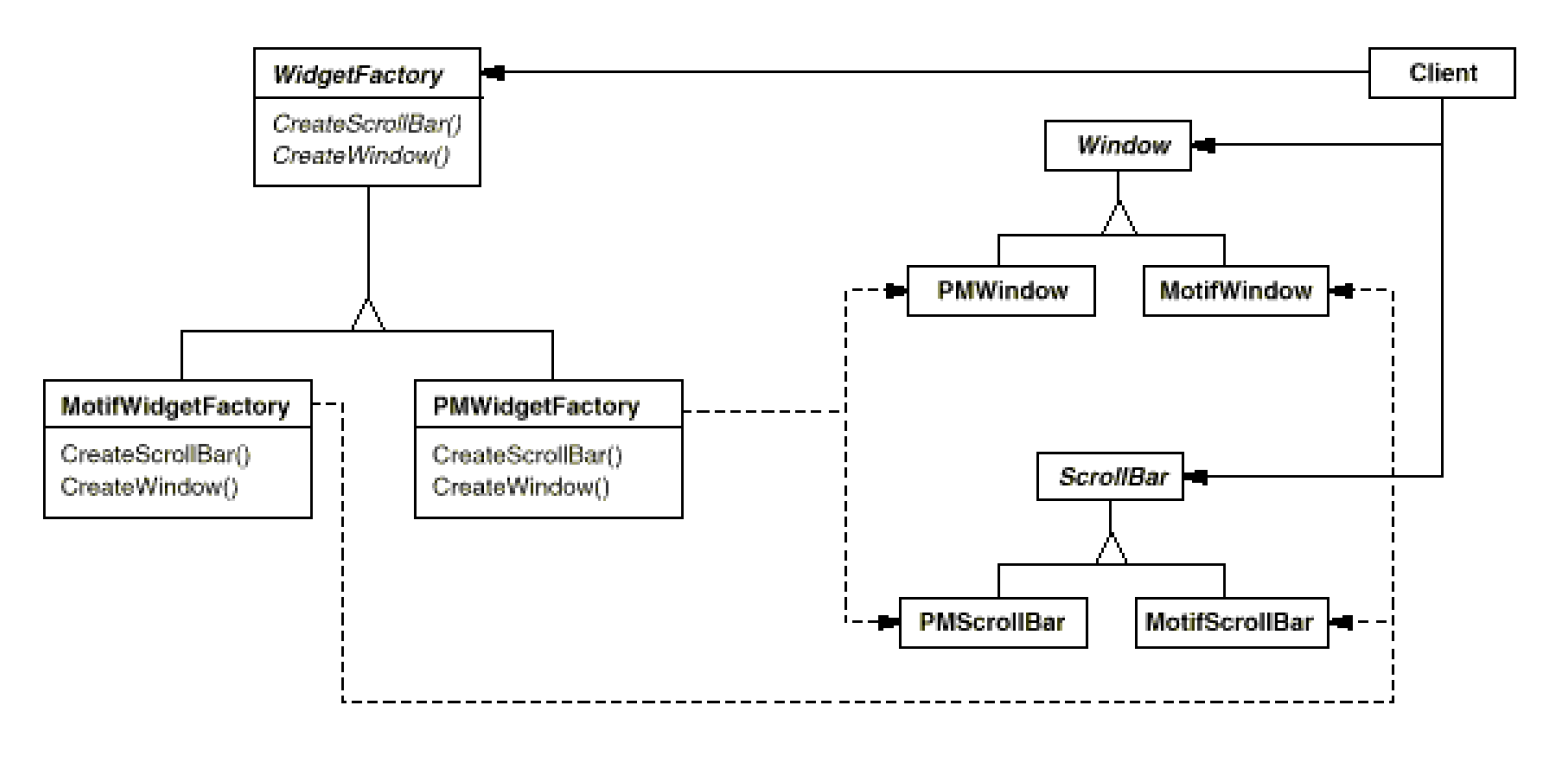
\includegraphics[scale=0.3]{motivation.png}
\end{center}
\end{frame}
%-------------------------------------------------------------------------------------------------

\subsection{Կիրառելիությունը}
%-------------------------------------------------------------------------------------------------
\begin{frame}\frametitle{Կիրառելիությունը}
Այս Ն.Ձ. պետք է օգտագործել երբ.
\vspace{0.5cm}
\begin{itemize}
    \item
    \item
\end{itemize}
\end{frame}
%-------------------------------------------------------------------------------------------------

\section{Կառուցվածքը}
%-------------------------------------------------------------------------------------------------
\begin{frame}\frametitle{Կառուցվածքը}
\begin{center}
    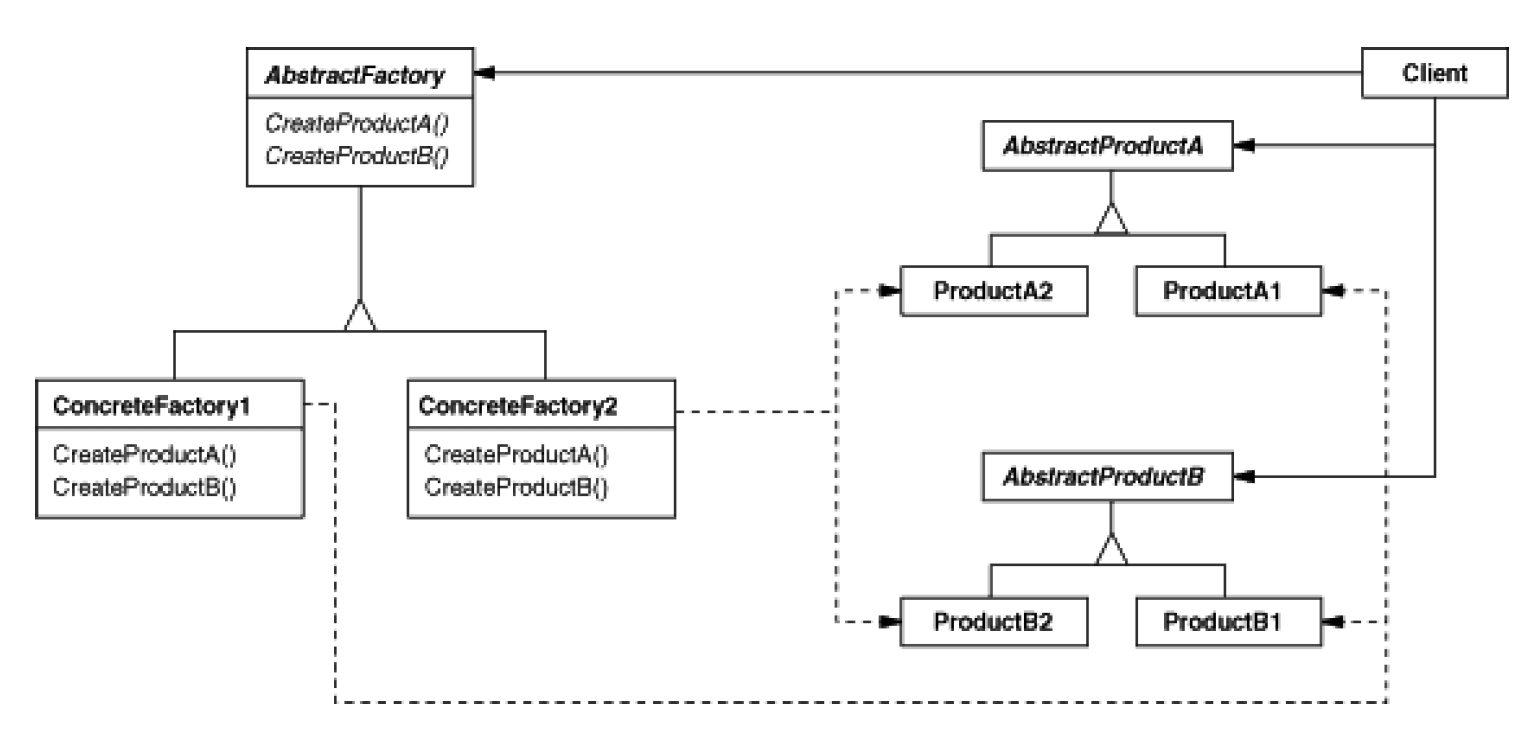
\includegraphics[scale=0.3]{structure.png}
\end{center}
\end{frame}
%-------------------------------------------------------------------------------------------------

\subsection{Հետևանքները}
%-------------------------------------------------------------------------------------------------
\begin{frame}\frametitle{Հետևանքները}
Այս Ն.Ձ. ունի հետևյալ առավելություններն ու թերությունները.
\vspace{0.5cm}
\begin{itemize}
    \item
    \item
\end{itemize}
\end{frame}
%-------------------------------------------------------------------------------------------------

\section{Իրականացումը}
%-------------------------------------------------------------------------------------------------
\begin{frame}\frametitle{Իրականացումը}
\begin{itemize}
    \item
    \item
\end{itemize}
\end{frame}
%-------------------------------------------------------------------------------------------------

\subsection{Օրինակ}
%-------------------------------------------------------------------------------------------------
\begin{frame}[fragile]\frametitle{Օրինակ}
\begin{english}
\begin{minted}{cpp}
    class Graphic {
        virtual void Draw(const Point& at) = 0;
        virtual void HandleMouse(Event& event) = 0;
    };
\end{minted}
\end{english}
\end{frame}
%-------------------------------------------------------------------------------------------------

\section{Առնչվող Ձևանմուշները}
%-------------------------------------------------------------------------------------------------
\begin{frame}\frametitle{Առնչվող Նախագծման Ձևանմուշները}
\begin{itemize}
    \item Adapter
    \item Decorator
\end{itemize}
\end{frame}
%-------------------------------------------------------------------------------------------------

\end{document}
